\chapter{Fundamentos LoRaWAN}

LoRaWAN es una \gls{wan} descrita en un modelo de tres capas: la de aplicación, la de control de acceso al medio (\gls{mac}) y la capa física o de transmisión, según se muestra en la figura \ref{f:m_protocolos}.

\begin{figure}[hb]
\centering
\caption{Capas de la red LoRaWAN}
\includegraphics[width =\textwidth]{capitulos/figuras/protocolos}
{\fuente{elaboración propia}}
\label{f:m_protocolos}
\end{figure}

\section{Capa Física}
En LoRaWAN, la capa física incluye la interfaz de radio, donde se diferencian las bandas \gls{ism} según la región, así como las técnicas de modulación \gls{fhss} y \gls{fsk}. En \gls{fhss}, el espectro se genera mediante una señal \gls{css} con variaciones continuas en la frecuencia. Esta técnica tiene la ventaja de que las compensaciones en tiempo y frecuencia son equivalentes.

Los sistemas \gls{fsk} y LoRa cuentan con modulación de envolvente constante, esquemas de bajo costo y baja potencia, con estados de alta eficiencia que pueden reutilizarse sin modificaciones. Gracias a la ganancia en procesamiento asociada a LoRa, la potencia de salida del transmisor puede reducirse y mantenerse comparable a la de un enlace convencional \gls{fsk}, al mismo tiempo que conserva o mejora las prestaciones del enlace.

El alto \gls{bt}, superior a 1, y su asincronismo natural hacen que la señal LoRa sea inmune a los mecanismos de interferencia tanto dentro como fuera de la banda. Además, proporciona excelente inmunidad frente a las interferencias de impulsos de amplitud (AM), ya que el periodo de símbolo de LoRa es más largo que las ráfagas de corta duración utilizadas en los saltos rápidos del sistema \gls{fhss}. Los valores típicos de selectividad fuera de canal son de 90~dB y el rechazo en el canal es superior a 20~dB. Los valores típicos para la modulación FSK son de 50~dB, con un rechazo de -6~dB.

El sistema también es resistente al efecto Doppler, el cual provoca pequeños desplazamientos en los pulsos LoRa, haciéndolos despreciables en el eje temporal de la señal en banda base.

Por estas razones, el sistema basado en LoRa es ideal para enlaces de comunicaciones de datos móviles, tales como sistemas de monitorización, aplicaciones de transporte, infraestructura, seguimiento, entre otros.

\section{Capa MAC} \label{secc:clases}

La capa \gls{mac} se compone de las subcapas LoRaWAN esclavo, \gls{hal} y \gls{spi}, y es la responsable de definir la clase del estándar que se implementará, pudiendo ser clase A, B o C. Este apartado aborda las especificaciones de la clase A de LoRaWAN. Asimismo, la capa \gls{mac} establece elementos clave para las redes, como la encriptación y la seguridad para \gls{m2m}, la optimización de la tasa de bits adaptativa, la calidad de servicio y otras aplicaciones avanzadas.

\subsection{LoRaWAN Clase A}

Los diferentes tipos de nodos se pueden implementar como clase A, con las capas física, MAC y de aplicación que constituyen el estándar. La definición de la clase se realiza en la capa \gls{mac}.

Una vez que el nodo transmite un mensaje, se abren dos ventanas de recepción de corta duración. La primera ventana, RX1, se activa tomando como referencia el final de la transmisión. 

\begin{figure*} 
    \centering
    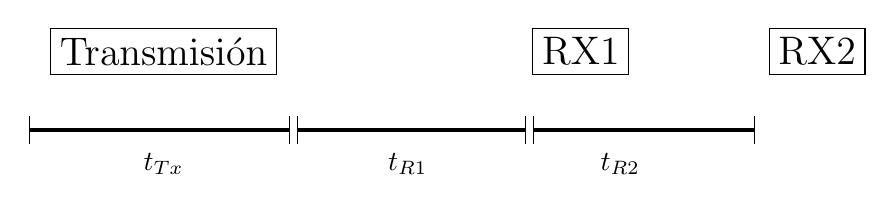
\begin{tikzpicture}
        \setlength{\arrayrulewidth}{0.2mm}
        \node[draw] at (1.7, 1)   (a) {\Large{Transmisión}};
        \node[draw] at (7, 1)   (b) {\Large{RX1}};
        \node[draw] at (10, 1)   (b) {\Large{RX2}};
        \draw [black, line width=0.05cm] (0cm, 0cm) -- (3.3cm, 0cm); 
        \foreach \x in {0, 3.3} 
        \draw (\x cm, 5pt) -- (\x cm, - 5pt); 
        \draw (1.7cm, 0cm) node[below=5pt] {$t_{Tx}$}; 
        
        \draw[black, line width=0.05cm] (3.4cm, 0cm) -- (6.3cm, 0cm);
        \foreach \x in {3.4, 6.3} 
        \draw (\x cm, 5pt) -- (\x cm, - 5pt); 
        \draw (4.8cm, 0cm) node[below=5pt] {$t_{R1}$};
        
        \draw [black, line width=0.05cm] (6.4cm, 0cm) -- (9.2cm, 0cm);
        \foreach \x in {6.4, 9.2} 
        \draw (\x cm, 5pt) -- (\x cm, - 5pt);
        \draw (7.5cm, 0cm) node[below=5pt] {$t_{R2}$};
    \end{tikzpicture} 
\caption{Tiempos de comunicación nodo-pasarela-nodo}
\label{f:retardo}
\end{figure*}

Esta \textbf{primera ventana} usa la frecuencia y la tasa de datos relacionadas con las características de la transmisión. La ventana RX1 se abre tras un retardo, $t_{R1}$, de aproximadamente \SI{20}{\us}, como se ilustra en la figura \ref{f:retardo}. Este retardo varía de acuerdo con las bandas regionales especificadas en los parámetros regionales de \gls{lwan}. Por defecto, la tasa de datos en RX1 es igual a la de la transmisión.

La \textbf{segunda ventana}, RX2, tiene parámetros de frecuencia y tasa de datos fijos, aunque pueden ser modificados mediante comandos \gls{mac}. El retardo $t_{R2}$ es de aproximadamente \SI{20}{\us}, como se muestra en la Figura\ref{f:retardo}. Los valores predeterminados de estos parámetros están definidos por las bandas regionales de los estándares \gls{lwan}.

La duración de la ventana de recepción debe ser al menos suficiente para que el transceptor del nodo pueda detectar el preámbulo del mensaje entrante.

\subsection{LoRaWAN Clase B}

Los nodos y la pasarela tienen comunicación bidireccional con ranuras de recepción programadas. Los nodos de clase B, además, tienen las funcionalidades de la clase A. Para alcanzar la sincronización de la red, los nodos reciben un tiempo de sincronización tipo Beacon desde la pasarela, esto permite al servidor saber cuándo un nodo está escuchando. Los nodos que hablen en la ventana de tiempo programada entran a la pasarela de acuerdo a procesos aleatorios con prioridad en servicios a los nodos en mención. 

\subsection{LoRaWAN Clase C}

Los nodos y la pasarela tienen comunicación bidireccional con ranuras de recepción máximas. Proporciona ventanas de recepción casi continuamente, solo se cierra cuando el nodo está transmitiendo. Este modo se utiliza cuando hay requerimiento de grandes cantidades de datos entre el nodo y la pasarela. 

\section{Tramas de transmisión y recepción}

Las tramas de la capa física se distinguen entre las de transmisión (\textit{uplink}) y las de recepción (\textit{downlink}), desde el punto de vista del nodo.

\begin{figure}
\caption{Estructura de tramas de \textit{uplink} y \textit{downlink}}
\centering
    \resizebox*{.8\textwidth}{2cm}{
    \begin{tabular}{|c|c|c|c|c|}  \hline
        \multicolumn{5}{|c|}{{\textbf{Estructura de transmisión} }}\\ \hline
         Preamble & PHDR & PHDR-CRC & PHYPayload & CRC \\ \hline \hline
         \multicolumn{5}{|c|}{{\textbf{Estructura de recepción} }}\\ \hline
         Preamble & PHDR & PHDR-CRC & PHYPayload& -- \\ \hline
    \end{tabular}}
\label{f:retardo1}
\end{figure}

\enlargethispage{-\baselineskip}

El nodo transmite la trama a la pasarela, figura \ref{f:retardo1}, y de ahí al servidor de red. La trama de la capa física de LoRa está compuesta por el preámbulo, el \gls{phdr}, el \gls{pc}, la carga útil (\textit{payload}) y el \gls{crc}. 

La trama de recepción la envía la pasarela a un solo nodo y es retransmitida por una única pasarela. Los mensajes de la capa física también se denominan modo explícito de paquetes de radio. Los mensajes de recepción tienen la misma estructura del mensaje de transmisión, a excepción del \gls{crc}, el cual está ausente, como se muestra en la parte baja de la figura \ref{f:retardo}.

La estructura de las tramas LoRa de la capa física contiene la información de las capas superiores (figura \ref{f:m_lora}), tal como lo es la capa \gls{mac}. El asterisco hace referencia a que el \gls{crc} solo está presente en la trama de transmisión.

\begin{figure}
    \caption{Formato del mensaje LoRa}
    \centering
    \includegraphics[width =\textwidth]{capitulos/figuras/f2}
    \label{f:m_lora}
\end{figure}

En la \gls{pp}, se encuentra el contenido de los diferentes tipos de tramas \gls{mac}, las cuales tienen en común el encabezado \gls{mhdr} y el \gls{mic}. Los tipos de tramas \gls{mac} corresponden a los de la \gls{mp}, solicitud de acceso (\textit{Join-Request}) y respuesta a la solicitud (\textit{Join-Response}). 

La trama \gls{mp} contiene la información de los nodos. Los campos de esta trama corresponden al \gls{fhdr}, \gls{fp} y a la \gls{fpa}. La \gls{fhdr} contiene los campos de \gls{da}, de \gls{fc}, de \gls{fcn} y las \gls{fo}.

\section{Características de LoRaWAN}

\textbf{Banda de frecuencias y canalización}. La banda EU-868 del estándar LoRa tiene un rango de \SI{863}{\MHz} a \SI{870}{\MHz} y también está definida en el espectro de radio para la banda \gls{ism} normatizada por \gls{etsi}, en el estándar EN300.220. Los canales de la red pueden ser atribuidos libremente por el operador. La pasarela posee ocho canales en paralelo, IF0 al IF7, como medio de comunicación con el nodo. El ancho de banda es fijo, 125~kHz, con tasa de bit variable de acuerdo al \gls{sf}.

\begin{figure}
    \caption{Canalización banda ISM868}
    \centering
    \includegraphics[width =\textwidth]{capitulos/figuras/canales}
    \label{f:m_canales}
\end{figure}

Además tiene dos canales adicionales, uno LoRa con ancho de banda fijo de 250 kHz con una tasa de bit de 11~kbps como el canal \textit{back-haul} de la red LoRaWAN IF1 y otro canal de \gls{gfsk}, el cual tiene una tasa de datos y un ancho de banda ajustables para una velocidad máxima de 50 kbit/s \cite{LoRa-2015}.

\textbf{Factor de ensanchado \gls{sf}, tasa de bit y potencia}. Permite un manejo eficiente del espectro y de la capacidad de la red LoRa. Hay seis factores de ensanchado \gls{sf}, que van del SF7 al SF12, los cuales están relacionados con la potencia y la tasa de datos. La tasa de datos va desde 250~bps, para \gls{sf}12 con una sensibilidad de recepción de -137~dBm, hasta 5.5~kbps, para \gls{sf}7 con una sensibilidad de -123~dBm. La potencia máxima de transmisión está, de acuerdo a \gls{etsi}, en 14~dBm. LoRa utiliza el ajuste dinámico de la potencia de emisión y la \gls{adr}, de acuerdo a la distancia que separa el nodo de la pasarela, de esta manera se maneja la eficiencia de la energía.

\section{Seguridad LoRaWAN}

La seguridad en LoRaWAN es uno de los activos más importantes en aplicaciones IoT, industriales, \gls{m2m}, ciudades inteligentes, etc. La seguridad cubre múltiples propiedades y en especial las criptográficas, las cuales merecen un estudio más profundo.  

La autenticación es bidireccional entre la red y el nodo para el flujo de los datos, una vez activado el nodo. Esto asegura que los nodos se unan y se autentiquen a la respectiva red. 
Los mensajes de aplicación de la capa \gls{mac} de LoRaWAN tienen autenticación de origen, integridad protegida, reproducción protegida y encriptación. Lo anterior unido a la autenticación mutua garantiza que el tráfico en la red no sea alterado y que proviene de un nodo legítimo de la red. Esto hace que la información no sea comprensible para los intrusos y tampoco permite ser capturada o alterada por los piratas. La tecnología LoRa es una de las pocas redes IoT que implementa encriptación de extremo a extremo.  
En las redes celulares el tráfico es encriptado en la interfaz de aire, pero es transportado como texto plano en el núcleo de la red del operador, lo cual puede ser vulnerado de forma selectiva. Para este problema se creó una etapa adicional para la seguridad. LoRaWAN no provee esta capa adicional ya que se aumentaría el consumo de potencia, la complejidad y los costos.

Potentes algoritmos de seguridad están implementados en la red LoRa como lo es el \gls{aes}, el cual ha sido adoptado para la seguridad del tráfico entre los nodos y la red en conjunto a los diferentes modos de operación como lo son: \gls{cmac} para proteger la integridad de la información y el \gls{crt} para la encriptación. Los nodos son personalizados con una clave \gls{aes} de 128~bit (AppKey) y un único identificador global (EUI-64-based DevEUI), figura \ref{f:seg1}. 

\begin{figure}
    \caption{Seguridad en la trama LoRaWAN}
    \centering
    \includegraphics[width =\textwidth]{capitulos/figuras/seguridad1}
    \label{f:seg1}
\end{figure}

La activación al aire (\textit{over-the-air}) provee el reconocimiento de ambos, el nodo y la red, por medio de la llave \textit{AppKey} el nodo se puede unir a la red, figura \ref{f:seg2}. Dos llaves de sesión que corresponden: una a la integridad del tráfico y la otra a la encriptación de los comandos y la carga útil de la aplicación de la capa \gls{mac} de \gls{lwan}  llamada \textit{NwkSKey}, y otra para la encriptación de extremo a extremo de la carga útil de la aplicación denominada \textit{AppSKey}. 

\begin{figure}
    \caption{Seguridad LoRaWAN}
    \centering
    \includegraphics[width =\textwidth]{capitulos/figuras/seguridad2}
    \label{f:seg2}
\end{figure}

La llave \textit{NwkSKey} es distribuida por la red LoRaWAN en su orden para probar y verificar la autenticidad y la integridad de los paquetes. La llave \textit{AppSKey} la provee el servidor de la aplicación para encriptar y desencriptar la carga útil de la aplicación. Las llaves, \textit{AppSKey} y \textit{AppKey}, están ocultas al operador de la red, por tal razón no se puede desencriptar la información del usuario.

\section{Capa de Aplicación}

Una \gls{wsn} es un sistema de comunicación conformado por varios nodos sensores, donde cada uno de ellos está dotado de los elementos apropiados para la detección de magnitudes físicas asociadas a procesos industriales, a la calidad del aire, al medio ambiente, o a otros eventos en la naturaleza.

La \gls{wsn} se ha hecho realidad por la convergencia de los desarrollos tecnológicos en los \gls{mems}, las comunicaciones inalámbricas y la electrónica digital.

La tecnología de miniaturización de los nodos para \gls{wsn}, basada en \gls{mems}, ha hecho un progreso notable en los últimos años.

La tecnología de \gls{mems} consiste en combinar la microelectrónica, el micromecanizado y el empaquetado en alta densidad.

Las estructuras en niveles 2D y 3D pueden ser producidas y soportadas por tecnologías de microelectrónica y micromecanizado, para pasar a formar parte de los sistemas sensores en miniatura, los cuales consumen baja potencia y llevan incluido directamente su sistema de acondicionamiento.

En este momento existe una gran variedad de productos \gls{mems} en el mercado, los cuales permiten la detección de una variedad de magnitudes en áreas de la física, la biología, la biomasa, entre otras. Entre dichas magnitudes se destacan los sensores para desplazamiento, velocidad, aceleración, presión, tensión, sonido, luz, variables eléctricas, variables termodinámicas, variables biológicas, y muchas más.

La tecnología de los \gls{mems} ha llegado, en este momento, a desarrollar nodos sensores de dimensiones del orden de $\SI{2}{mm}\times \SI{2}{mm}\times \SI{1}{mm}$.

La combinación de \gls{iot} y \gls{wsn} permite un desarrollo revolucionario de los sistemas de comunicación con mejoras en la confiabilidad, flexibilidad, cubrimiento y eficiencia.

La \gls{wsn} está configurada por una red de nodos que cooperativamente sensan y controlan un medio, lo que permite la interacción entre las personas o los sistemas de cómputo y el entorno \cite{Akyildiz-2002}.

La actividad de detección, procesamiento y comunicación está limitada por la cantidad de energía disponible, lo cual exige un diseño integral que conlleva procesamiento de señales, control de acceso al medio y protocolos de comunicación.

Las aplicaciones de la tecnología \gls{wsn} permiten el desarrollo de sistemas inteligentes en áreas tales como manejo de aguas, transporte, hogar, industria, entre otras y siempre con mejoras importantes sobre las tecnologías tradicionales.

Agregado a lo anterior, el mundo moderno de las \gls{wsn} emigra hacia una nueva era con su integración al \gls{iot}, donde habrá una gran variedad de temas que deberán ser normados y aceptados en un corto tiempo. Algunos de estos temas más apremiantes son la propiedad, uso y legalidad de los datos que se generan, directa o indirectamente, gracias a dichos sistemas.

En su estructura fundamental, una \gls{wsn} está constituida por:
\begin{itemize}
\item Los nodos sensores dispuestos para detección de las diferentes magnitudes y para la comunicación.
\item Los nodos actuadores, los cuales ejecutan funciones de control comandadas de acuerdo al resultado de una medición previa.
\item La pasarela o gateway encargada de la conexión a internet.
\item Los clientes. 
\end{itemize}

Los nodos transmiten y reciben el estado de cada uno de ellos entre sí para reconocerse como existentes en la red. Los nodos configuran una red (estrella, o malla, o cualquier otra) con cubrimiento de distancias cortas con un máximo de 1000~metros y utilizando la técnica multi-salto. 

\newpage\thispagestyle{empty}
